% Load required classes and packages
\documentclass{mxl-note}
\usepackage{listings}

% Set up document variables
\begin{document}
\title{Mercury2 Design Document}
\author{Jimmy Blanchard, Tatyana Dobreva}
\docnum{0.2.3}
\setcounter{secnumdepth}{5}

% Table of Contents
\maketitle
\tableofcontents
\newpage 

% Definitions
\section{Definitions} 
Several of the most commonly used words and acronyms in this document are defined below.

\begin{table}[h]
	\footnotesize {\begin{tabular}{ p{5cm} p{10cm} }
		\textbf{Mercury2} & Colloquially refers to the complete set of ground station applications (the web interface and Iris ground station service). More specifically refers to just the web application that controls Iris instances.\\[.2cm]
		\textbf{Iris} & A ground station service application that runs on a computer attached to the pipeline hardware.\\[.2cm]
		\textbf{Hardware Pipeline} & A collection of related hardware used to either transmit or receive information to and from the radio (or both, if the hardware supports it).\\[.2cm]
		\textbf{Ground Station} & Refers to a Mercury2 installation and all Iris instances configured to use it. Generally, this means several computers and pieces of hardware on the same local area network.\\[.2cm]
		\textbf{Satellite} & A device in orbit that Iris configured radios can connect to.\\[.2cm]
		\textbf{Pass} & A transit of a satellite over a Iris configured ground station. Passes can be scheduled, which reserves an Iris instance for the duration of the pass. Scheduled passes are identified by the satellite name, orbit number, and ground station.\\[.2cm]
		\textbf{Timestamp} & The duration of scheduled usage sessions for Iris instances will be defined by a start and end timestamp. These timestamps will be simple UNIX timestamps indicating the start and end of the reservation.\\[.2cm]
		\textbf{Satellite Operator} & An entity that remotely reserves ground station access and uses it to connect to a satellite.\\[.2cm]
		\textbf{Ground Station Operator} & A user that is granted some management privileges over the ground station. For example, the ability to approve or deny reservation requests and the ability to modify the upcoming pass schedule.\\[.2cm]
		\textbf{Ground Station Administrator} & A user with complete administrative control over the ground station.\\[.2cm]
		\textbf{MVC Framework} & Model-View-Controller framework. Refers to a common web application software design pattern.\\[.2cm]
		\textbf{YAML} & An easy-to-use configuration format. Will be used to configure Iris ground stations.\\[.2cm]
	\end{tabular}}
	\caption{General Definitions}
	\label{tab:myfirsttable}
\end{table}

% Introduction
\newpage
\section{Introduction}
Mercury2 is the spiritual successor to the Mercury Ground Station System. It will allow satellite operators to automatically reserve and configure ground stations, while at the same time still giving ground station operators complete control over their hardware. Mercury2 will include a feature rich cross-platform web interface. Eventually, it will help enable a global federated ground station network.

% Requirements
\section{Requirements}
Mercury2 must be able to perform several core functions. It will consist of two separate applications: Mercury2 (the web interface), and Iris (ground station daemon). In addition, each Iris instance can support multiple hardware drivers. Their core requirements are defined below.

\subsection{Mercury2 Requirements}
Mercury2 will run on an web accessible server (that can be seperate from the computers that Iris runs on).
\begin{itemize}
	\item User authentication and authorization
		\begin{itemize}
			\item Supports user registrations and account management
			\item Maintains user permissions
		\end{itemize}
	\item Complete access logs
	\item Satellite operator interface
		\begin{itemize}
			\item Reserve ground station use during a specified time window
			\item View history of previous passes
			\item Configure ground station during pass
			\item Access sockets forwarded from Iris instance
		\end{itemize}
	\item Ground station operator interface
		\begin{itemize}
			\item Add and edit Iris instances and associated drivers
			\item View and modify ground station schedules
			\item Ability to approve or deny pass requests
			\item Manually download schedules and upload results if the ground station is not web-enabled
			\item Manual override to disable automatic scheduling and give ground station operator direct control
		\end{itemize}
	\item Complete administration panel
	\item Easy to use interface
	\item SSL encryption and protection from exploits such as XSS cross-site scripting and SQL injection 
\end{itemize}

\subsection{Iris Requirements}
An instance of Iris will run on a computer attached to each ground station radio. Mercury2 may have multiple instances of Iris and their drivers associated with it. Iris will:
\begin{itemize}
	\item Support multiple radio drivers using a generalized interface
	\item Periodically connect to Mercury2 to download pass schedule and connection settings
	\item Provide satellite operators with a TCP socket to send and receive data from the satellite , and command the ground station
	\item Automatically initialize sockets when a pass starts
	\item Secure, private key verified transmissions
	\item Maintain copies of all telemetry data received
\end{itemize}

\subsection{Driver Requirements}
Drivers allow Iris to interface with a wide range of hardware configurations. By interpreting ground station commands sent to Iris from Mercury 2, drivers will also give operators direct control over the ground station.
\begin{itemize}
	\item Define functionality driver exposes (and in turn the commands that it responds to) via configuration file
	\item Send incoming satellite command data to radio
	\item Forward telemetry data to Iris (which puts it on a socket) from the radio
	\item Parse and respond to supported ground station commands
\end{itemize}

% Architecture Design
\clearpage 
\section{Application Architecture}
\begin{figure}[hbtp]
\centering
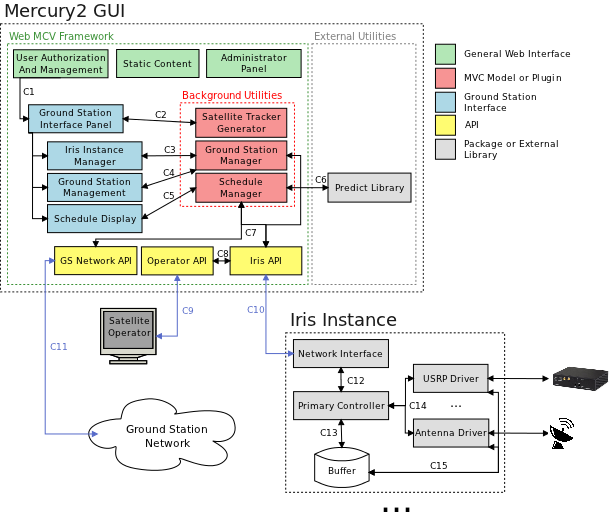
\includegraphics[scale=.60]{Architecture_Overview.png}
\caption{Mercury2 and Iris Architecture Overview}
\end{figure}

% Mercury2 GUI Architecture
\subsection{Mercury2 GUI}
The Mercury2 GUI will most likely be a PHP based web MVC framework (e.g. CodeIgniter, CakePHP). An application following this design pattern is broken into models (handle database interactions and various logic tasks), views (the mark up used to display content to the user), and controllers (classes that route users to the appropriate location and join models and views). Figure 1 (above) roughly illustrates the various components that will be used in the application. Each component is explained below. 

\subsubsection{User Authorization and Management}
\begin{description}
	\item [Controller Class]UserController
\end{description}
This section of the website is responsible for managing users and user permissions. It performs several standard user functions, such as account editing, sign-ups, and password recovery. Account creation will be free and open to the public (except, perhaps, in the case of for-profit groups, for which a tiered priced system could be implemented). The ground station operator will be able to specify whether or not each new account needs to be approved by an administrator. Once their account has been created and approved, satellite operators will be able to schedule use of any configured Iris instance.

\paragraph{User Groups}
This controller will also allow users to create custom user groups and add other users to it. These groups will allow satellite operators to create a "team" of users on Mercury2 that can share scheduling information, view shared session pages, and use each other's saved session settings (e.g. tracking information, hardware settings, etc.) when scheduling new satellite passes.

\subsubsection{Static Content}
\begin{description}
	\item [Controller Class]ContentController
\end{description}
This will simply display administrator editable static content to the user such as the FAQs, API documentation, and Terms of Service.

\subsubsection{Administrator Panel}
\begin{description}
	\item [Controller Class]AdminController
\end{description}
The administrator panel will allow ground station administrators to manage Mercury2 and Iris instances. In addition to being able to do anything that any other appropriately permissioned user can do (such as viewing signal data, pass schedules, etc.), administrators will be able to:
\begin{itemize}
	\item Manage users and user permissions
	\item Configure website settings
	\item Create and edit static content
	\item Add and manage Iris instances (and associated drivers)
	\item Manage Iris API keys
	\item View application and API statistics
\end{itemize}

%% Ground Station Interface
\subsubsection{Ground Station Interface Panel}
\begin{description}
	\item [Controller Class]StationController
\end{description}
Each configured Iris instance will receive its own set of pages on Mercury2. These pages will be customized based on who is viewing them and the functionality of the selected Iris instance. Satellite and ground station operators will be able to control the ground station from these pages. Note that the ground station interface panels and schedules are defined per Iris instance. That is, each instance of Iris added to Mercury2 is effectively its own ground station.
\paragraph{Weather Override} This feature will safeguard the operators from scheduling during interfering weather such a thunderstorms, lightning, snow storms, and heavy rain. During the ground station setup, the ground station operators will specify the location which will then be used to query various online weather services to determine the risk of hazardous weather.

\paragraph{Common Features} There will be several features that can be displayed regardless of who is viewing the page. These are:
\begin{itemize}
	\item List of upcoming passes
	\item Upcoming usage schedule
	\item Satellite tracker and Az/El chart
	\item Ground station status
\end{itemize}

\paragraph{Ground Station Operators} Ground station operators will have the highest degree of control over any given Iris instance. From the ground station interface panels they will be able to perform several tasks, which are listed below.
\begin{itemize}
	\item View complete pass schedule
	\item View pass history
	\item Configure which of the common features (defined above) are active (and for who)
	\item Approve or deny ground station reservation requests (if enabled)
	\item Manually add, edit, or remove upcoming passes
	\item Manually issue commands to the Iris instance
	\item View complete ground station health
	\item Communicate with satellite operators via private message
	\item Assume manual control of the ground station and remove it from the scheduling pool
	\item Download raw copy of the pass schedule if Iris instance is in offline mode
\end{itemize}

Note that manual control of a ground station is similar to scheduled passes. When manual control is requested, the schedule is modified to include the request, which is then interpreted by the selected Iris instance when the schedules are synced. The ground station operator will then be presented with a session page containing the socket connection settings (described below in section 4.1.4.4).

\paragraph{Satellite Operators} When a satellite operator visits an Iris interface panel, they will be able to perform the following tasks.
\begin{itemize}
	\item View upcoming passes at the ground station
	\item Send a private message to or initiate a chat with the ground station operators
	\item Reserve or request an Iris pipeline for a specified pass or time
		\begin{itemize}
			\item Specify radio settings to use during pass
			\item Request priority if Iris instance all ready reserved (for emergencies, etc.)
			\item Specify driver specific initialization parameters such as tracking information and switch settings (which are presented using custom view partials for each driver in the pipeline)
		\end{itemize}
\end{itemize}
When a satellite operator schedules a pass, the settings they specify will be recorded and can be loaded when they want to schedule a pass again. This will allow for easy scheduling of repeated passes by the same satellite. Each pass scheduled will be given its own page that is known only to the satellite operator(s) that scheduled it (or ground station operators). From this sub-page, satellite operators will be able to:
\begin{itemize}
	\item View socket connection settings (unique for each scheduled pass)
	\item View active Iris instance and driver health
	\item View streaming signal data (e.g. waterfall plot) if connection permits
	\item Issue commands to the ground station
		\begin{itemize}
			\item The commands available to the satellite operator are set by the radio drivers and ground station operators
			\item Each command interface is rendered using a custom HTML view partial
		\end{itemize}
\end{itemize}

%% APIs
\subsubsection{Iris API}
\begin{description}
	\item [Controller Class]IrisAPIController
\end{description}
The IrisAPIController will provide API hooks that will allow Iris instances to download schedules, report their health and status, receive ground station commands, and forward the radio communication sockets to the satellite operator (via the Operator API, explained in the next section). The API will consist of a standard RESTful route scheme combined with sockets and is explained fully in section 4.3.9.

\paragraph{Conflicting Ports}
Because different Iris instances can be used at the same time, the socket ports used to connect to them to Mercury2 must be unique and tied to each scheduled pass. In addition, the sockets will need to be closed after each pass ends. This could be achieved using a simple CRON job.

\subsubsection{Operator API}
\begin{description}
	\item [Controller Class]OperatorAPIController
\end{description}
This API simply forwards the radio communication sockets from the active Iris instance to the satellite operator. Note that because the Iris API sockets are at the same level, the sockets exposed by the Operator API must use a different port to avoid conflicts. All of these ports will be determined automatically when the pass is scheduled.

\subsubsection{GS Network API}
\begin{description}
	\item [Controller Class]To Be Determined
\end{description}
This API will allow for eventual integration with the planned ground station network. It will allow for user sharing, schedule syncing, and remote ground station configuration, among other things.

%% Background Utilities
\subsubsection{Background Utility: Satellite Tracker Generator}
\begin{description}
	\item [Controller Class]TrackerController
\end{description}
This controller will support an internal API that will provide the necessary framework and configuration settings for instances of the satellite tracker and AZ/EL chart on satellite and ground station pages. Explained more in section 4.3.2.

\subsubsection{Background Utility: Schedule Manager}
\begin{description}
	\item [Model Class]Schedule
\end{description}
The schedule manager will be responsible for managing the requests for Iris instance use by satellite and ground station operators. It will ensure that only one satellite is using any given Iris instance at a time. All signal and telemetry data collected will be tied to a specified scheduled pass. The complete scheduling request and execution flow (including Iris interactions) is described below in figure 2.
\begin{figure}[hbtp]
\centering
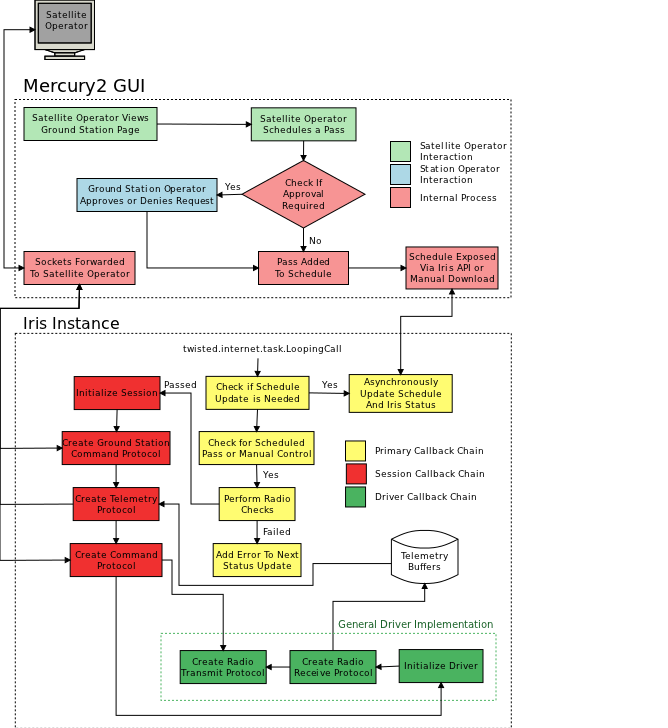
\includegraphics[scale=.65]{Pass_Flow.png}
\caption{Scheduled pass flow}
\end{figure}

\paragraph{Socket Ports}Each Iris instance must provide TCP sockets to enable satellite operators to directly control the satellite and receive telemetry data. This may result in connection overlap between sequential passes (because generally the ground station internet connection can't stream the telemetry data as fast as it's received). Thus, each pass will require unique socket ports. This will allow a scheduled pass to occur while the results of the last pass are still being streamed. This is described more in section 4.2.2.

\subsubsection{Background Utility: Ground Station Manager}
\begin{description}
	\item [Model Class]Stations
\end{description}
The ground station manager model is responsible for managing Iris instances and their associated drivers. It will record driver capabilities and available commands for use in the Ground Station Interface Panel.

\subsubsection{External Utility: Predict Library}
\begin{description}
	\item [Type]External API
\end{description} 
Mercury2 will make use of, at least initially, the popular \textit{Predict Library}\footnote{http://www.qsl.net/kd2bd/predict.html} by John Magliacane to calculate pass times. \textit{Predict} provides an API via a network socket that will allow Mercury2 to pass it TLE's and retrieve calculated pass times.

% Iris Task Manager Architecture
\subsection{Iris Task Manager}
The Iris Task Manager program will consist of a relatively simple Python script running on a computer connected to the radio. It will be primarily responsible for syncing schedules with Mercury2, configuring radios as needed, providing command (satellite and ground station) and telemetry sockets, and reporting ground station health. It will be built on top of Twisted, an asynchronous event driven network framework.

\subsubsection{Network Interface}
All network connections in Iris will be managed by Twisted. Twisted represents each connection made with users or the radios as an instance of a "Protocol" class, which asynchronously responds to network events as they occur. Each network connection will require its own protocol class, which will be constructed as needed. Iris will also use standard HTTP POST to periodically report its health and retrieve its schedule from Mercury2's REST API (described in sections 4.1.5 and 4.3.9). 

\paragraph{Network Security}
To ensure secure communication, all interactions between Iris and Mercury2 will be encrypted with a standard SSL encryption scheme. In addition, all communications with Mercury2 will need to be verified using a HMAC-SHA256 private key encryption system which will ensure only the authorized ground stations can access the API at any given time.

\subsubsection{Primary Controller}
The primary Iris module will initialize the program and create the main program loop (using \textit{twisted.internet.task.LoopingCall}). This "main loop" will responsible for maintaining the program state and coordinating Twisted callback chains. Its responsibilities will include: 
\begin{description}
	\item [Report Status and Fetch Schedules] Periodically (every minute or so) asynchronously POST the ground station's status (active task, radio parameters, etc.) to Mercury2's REST API (described in section 4.3.9), which responds with the ground station's most recent schedule. 
	\item [Execute Scheduled Passes] Once a scheduled pass starts (or once a manual control request is detected), Iris will:
		\begin{itemize}
			\item Construct an instance of the Session class (represents scheduled events)
			\item The new Session object would then construct an instance of the ground station command, satellite telemetry, and satellite command protocols on the ports specified by the schedule
			\item The Session would then create an instance of the radio driver class which would in turn create an instance of the radio protocol
			\item Update the application state with the active task
		\end{itemize}
	\item [Complete Scheduled Passes] Once a pass has finished (determined by the schedule), Iris will:
		\begin{itemize}
			\item Update the application state with the completed task
			\item Destroy session and protocol objects when the pass is over and all of the telemetry has been transmitted
		\end{itemize}
\end{description}

\paragraph{Application State} The Iris application state will be maintained in a singleton class initiated at runtime. This class will be used to store, access, and modify all of the Iris state, including:
\begin{itemize}
	\item Most recent version of the schedule from Mercury2
	\item Currently executing task
	\item Hardware pipeline status
	\item Status messages (e.g. "Event failed", "Event cancelled by administrator", "Event cancelled by inclement weather", etc.) with associated event IDs
	\item Ground station configuration (loaded at runtime)
	\item Connection settings (e.g. Mercury2 IP address)
\end{itemize}
The state class will provide access methods for updating these values and generating a representation of the state to send to Mercury2 (most likely JSON). Note that in this model, all scheduling information is stored persistently in the Mercury2 database (and Iris just receives a copy). Iris configuration settings will be stored in a YAML configuration file that is loaded and initialized into the application state when Iris starts.

\subsubsection{Hardware Drivers}
Each hardware device present at a ground station will require its own "driver" class in Iris. The amount of functionality exposed by hardware drivers is dependent on what the hardware supports. At the very least, a hardware driver must provide an access method to retrieve the current state of the hardware (e.g. power settings, health, frequency, etc.). More complex drivers, such as radio drivers, will also need to provide the means to record and pass on any telemetry or command data. This will be achieved by using a series of file/memory buffers to pass information between the network interface and the active driver. Every hardware driver will have a configuration file which will define the ground station commands that it responds to (e.g. "Power On", "Power Off", "Set Frequency", etc.).  As ground station commands come in from the network interface, they will trickle down the active hardware pipeline (section 4.2.4) until a device driver successfully responds to it. Drivers must be designed in an asynchronous fashion as to prevent blocking. In practice, this means using Twisted Protocols to respond to hardware events. 

\paragraph{Telemetry Buffer} All satellite telemetry collected by Iris via the radio will be stored directly into a buffer file (unique for each session). After the radio driver receives a chunk of information from the radio, it will store it in the buffer file and notify the telemetry protocol (maintains the telemetry socket to the satellite operator) that more information is available for transmission. This achieves two things. First, it provides a redundant copy of the telemetry information in case the connection with the satellite operator is lost or the ground station is in offline mode. Second, it allows the radio to download information faster than it can send it to the satellite operator. This will prevent data from being lost if the internet connection is slow. A similar buffer will be used to store incoming satellite commands from the satellite operator and relay them to the radio protocol.

\paragraph{Telemetry Persistence}
All of the telemetry data collected will be stored in a file for a certain period, in case there was an error transmitting or receiving it the first time. This will also allow operators running ground stations without internet access the ability to manually retrieve the telemetry from a pass and send it to satellite operators.

\subsubsection{Hardware Pipelines}
Because there is such a large variety in possible ground station configurations, ground station administrators will define "hardware pipelines" in the Iris configuration that specify which pieces of hardware can be used together, along with any initial hardware state (e.g. power on each device, set the default antenna positions, etc.). Satellite operators will reserve Iris use per pipeline. That is to say, when making reservations they will select which hardware pipeline they want to use. Because there is often a difference between the hardware used to transmit and receive to and from the satellite, seperate "transmit" and "receive" pipelines will be defined. In addition, "transceive" pipelines (that allow simultaneous transmission and receiving) can be defined. 

\subsubsection{Offline Mode}
Because an Iris instance may not always have a reliable internet connection (e.g. if it's in a remote location), it can be configured to work in offline mode. In offline mode, the ground station staff would run the Mercury2 GUI on a remote web-accessible server. This will allow satellite operators to reserve radio use and specify hardware settings like a normal web-enabled Iris instance. However, because the actual Iris instance won't be accessible to the satellite operator when the scheduled event starts, they would need to upload a file containing the information they want transmitted when they create the schedule (or otherwise get it to the ground station operator). The ground station operator would then copy the schedule and transmission file to the computer running the Iris instance. Iris would then load it's schedule from the offline file and transmit the specified files when the time comes. The ground station operator would then be responsible for copying and sending the received telemetry information to the satellite operator at a later time. 

\subsection{Connection Details}
The connections shown in figure 1 (labeled C\#) are the primary data routes for the Mercury2/Iris system. They are explained in detail below.

\subsubsection{C1 - User Authorization}
\begin{description}
	\item [Connection Type] Database Model Interaction
\end{description}
When a user requests an Iris instance page in their browser, their permissions will be retrieved from the database to determine what features, if any, they will be able to use. Users can be given an arbitrary amount of control over any ground station by either website administrators or ground station operators. This will allow ground station operators to task multiple users with managing the ground station. In addition, users and ground station operators will be able to create user groups to allow multiple users to easily schedule passes and manage ground stations.

\subsubsection{C2 - Satellite Tracker Tool}
\begin{description}
	\item [Connection Type] Database Model Interaction
\end{description}
When a ground station page contains an instance of a satellite tracker, it will use the satellite tracker generator (section 4.1.8) to generate the appropriate configuration for that tracker (e.g. available satellites, ground stations, visual options, etc.). By seperating the tracker configuration generation from the satellite and ground station controllers, it is much more modular and can be included in any configuration on any arbitrary page.

\subsubsection{C3,C4 - Ground Station Manager}
\begin{description}
	\item [Connection Type] Database Model Interaction
\end{description}
The Iris Instance and Ground Station management panels will both use the Station model to retrieve information about the active Iris instance (and its associated drivers) from the database. In addition, the ground station health and status from the Iris API will be exposed via these connections.

\subsubsection{C5 - Schedule Manager}
\begin{description}
	\item [Connection Type] Database Model Interaction
\end{description}
These connections will allow any page on Mercury2 (particularly the ground station interface panels) to view a subset of the pass schedule. For example, when a user loads a ground station interface page the schedule manager will be queried, through this connection, for the relevant pass schedule. This connection will also allow authorized users to add passes to the schedule or cancel upcoming passes.

\subsubsection{C6 - Predict Library API}
\begin{description}
	\item [Connection Type] External API Connection
\end{description}
Mercury2 will use the \textit{Predict Library} (section 4.1.11) to calculate the times of upcoming passes. \textit{Predict} is a C application that runs independent of the Mercury2 MVC framework server application. \textit{Predict} provides a TCP socket based API that will allow the Mercury2 schedule manager to load current TLE's and retrieve upcoming passes.

\subsubsection{C7 - Internal API Connections}
\begin{description}
	\item [Connection Type] Database Model and Controller Interactions
\end{description}
The connections between the various APIs and internal database models will facilitate passing information such as the ground station schedule to the APIs, and in turn to any given Iris instance or to the ground station network.

\subsubsection{C8 - Iris Socket Forwards}
\begin{description}
	\item [Connection Type] Controller Interaction
\end{description}
This connection will be used to forward the LAN command and telemetry sockets provided by Iris to sockets accessible by the satellite operator. 

\subsubsection{C9 - Satellite Operator API}
\begin{description}
	\item [Connection Type] External API Connection
\end{description}
This API will allow satellite operators to access the command and telemetry sockets from Iris that were forwarded through Mercury2.

\subsubsection{C10 - Ground Station API}
\begin{description}
	\item [Connection Type] External API Connection
\end{description}
This API will be used by any configured Iris instance to connect to Mercury2. It will allow Iris instances to retrieve the most recent version of their schedules, report their health and status, and stream signal data back to Mercury2. In addition the various command and telemetry sockets will be forwarded through this API before they are exposed to satellite operators. Schedule and status updates will be done through a standard REST API, which is defined below.
\begin{description}
	\item [/api/schedule/:station-name.format] The ground station will POST to this path with its current health and status (a representation of the state class described in section 4.2.2.1). The Mercury2 API will respond with a .format (either JSON or XML) encoded string containing the ground station's schedule and radio connection settings for each scheduled event. It will also transmit a checksum to allow the ground station to verify the integrity of the transmission.
\end{description}

\paragraph{API Security}
API connection security will consist of standard SSL encryption to protect against middle-man attacks and HMAC-SHA256 private key encryption to prevent unauthorized access. Ground station operators will be able to generate and retrieve API keys from the ground station interface page.

\subsubsection{C11 - Ground Station Network API}
\begin{description}
	\item [Connection Type] External API Connection
\end{description}
This API will allow for eventual integration with the planned Ground Station Network. It will enable several features including shared users, schedule syncing and optimization, and remote ground station configuration. This interface will be defined at a later date.

\subsubsection{C12 - Primary Controller and Network Interface Interaction}
\begin{description}
	\item [Connection Type] Internal Connection
\end{description}
The primary application loop (section 4.2.2) will interface with the network interface package of classes (composed of Twisted protocols) to handle all network connections with Mercury2 and satellite operators.

\subsubsection{C13,C15 - Socket Buffer}
\begin{description}
	\item [Connection Type] Internal Connection
\end{description}
All telemetry and command data received from both the satellite and satellite operators will be stored in session-specific (i.e. each session gets its own set of files) buffer files. As explained in section 4.2.3.1, this will allow for telemetry redundancy and backups as well as a network buffer to facilitate slower connection speeds. Because the telemetry data collected per pass can be very large (on the order of gigabytes) and quickly fill up a harddrive, ground station administrators will be able to specify how long these files should be kept for before rotating them out.

\paragraph{Communication Between Protocols}
Each device or network interface in Iris will be defined by a Twisted Protocol class. These classes will respond to network events (e.g. "data received" or "connection opened") and act accordingly. Because the Twisted event-driven design pattern is asynchronous, these protocols must have a way to pass information between each other. For the telemetry stream, this will entail the radio protocol writing the information to the session's telemetry buffer file (explained in 4.2.3.1) as it streams in from the radio, and instructing the telemetry protocol (maintains telemetry socket to the satellite operator) that more information is available, which would cause it to read and transmit the new information from the buffer to the satellite operator via the telemetry socket. This is similar to how satellite commands will be transmitted from the satellite operator to the radio via the radio protocol. Ground station commands will be sent to Iris from either Mercury2 (via interface forms) or directly by satellite operators. Once these commands are received by the ground station command protocol, they will be parsed using a Iris utility function and then passed to the active session for hardware specific processing.

\subsubsection{C14 - Driver Interface}
\begin{description}
	\item [Connection Type] Internal Connection
\end{description}
The primary controller will connect to each hardware driver using a standard class interface (explained in section 4.2.3. This will provide the mechanism to allow the ground station to configure the hardware settings, as defined by the pass schedule, and respond to ground station commands sent from Mercury2.

\end{document}
